\subsection{Course Information}

\begin{frame}{\myframetitle}
	\begin{note}{Who Are We?}
		\centering
		\parbox{0.45\linewidth}{
			\centering
			\href{https://www.dbse.ovgu.de/Mitarbeiter/Gunter+Saake.html}{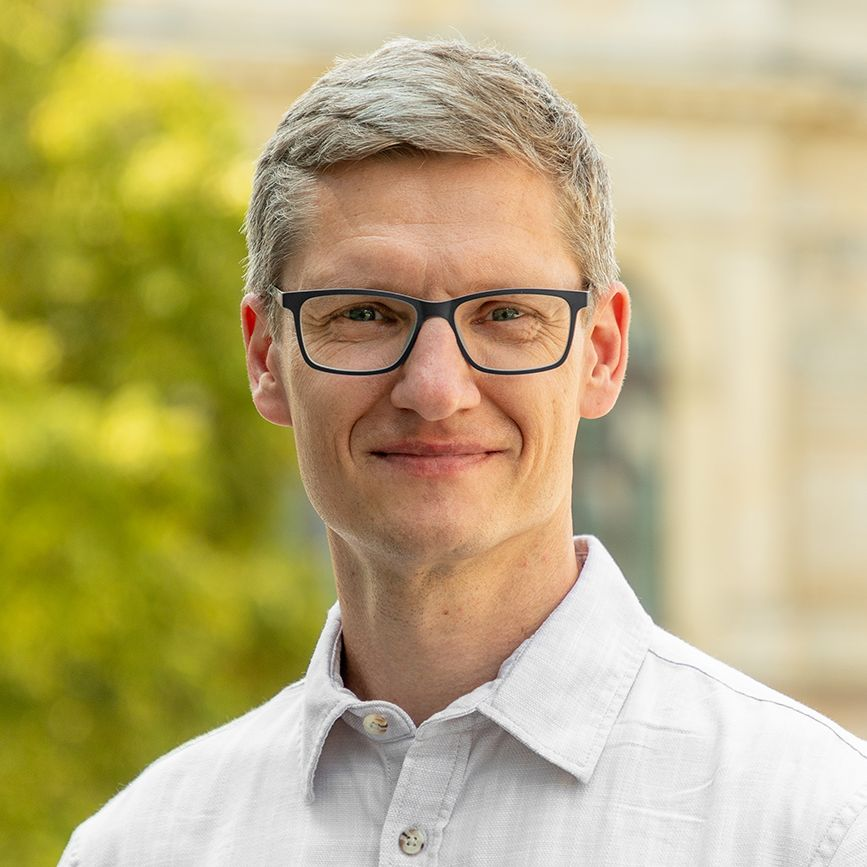
\includegraphics[height=5cm]{thomas-thuem}}\\[.5ex]
			\href{https://www.dbse.ovgu.de/Mitarbeiter/Gunter+Saake.html}{\emph{Thomas Thüm}}\\[.5ex]
			\small professor for software engineering\\[.5ex]
			FeatureIDE head
		}
		\parbox{0.45\linewidth}{
			\centering
			\href{https://www.dbse.ovgu.de/Mitarbeiter/Elias+Kuiter.html}{
\includegraphics[height=5cm]{chico-sundermann}}\\[.5ex]
			\href{https://www.dbse.ovgu.de/Mitarbeiter/Elias+Kuiter.html}{\emph{Chico Sundermann}}\\[.5ex]
			\small PhD student in feature-model analysis\\[.5ex]
			FeatureIDE core developer
		}
	\end{note}
\end{frame}

\subsection{Lectures and Exercises}

\begin{frame}{\myframetitle}
	\begin{mycolumns}
		\begin{definition}{Lecture}
			\begin{itemize}
				\item once per week
				\begin{itemize}
					\item on \emph{Thursday}, 12:15--13:45
					\item in room O27/123
					\item next lecture 20.04.
				\end{itemize}
				\item usually held by Thomas
				\item \emph{slides} are available on \texttt{\href{https://moodle.uni-ulm.de/course/view.php?id=37352}{Moodle}}
				\item \emph{guest lectures} planned
			\end{itemize}
		\end{definition}
	\mynextcolumn
		\begin{example}{Exercise}
			\begin{itemize}
				\item once per week
				\begin{itemize}
					\item on \emph{Tuesday}, 90 minutes in 10:00-12:00?
					\item in room O28/H21
					\item starts on 25.04.
				\end{itemize}
				\item usually held by Chico
				\item exercise sheets are available on \texttt{\href{https://moodle.uni-ulm.de/course/view.php?id=37352}{Moodle}}
				\begin{itemize}
					\item \emph{theoretical tasks}
					\item \emph{practical tasks}
				\end{itemize}
			\end{itemize}
		\end{example}
	\end{mycolumns}
\end{frame}

%\subsection{Practical Tasks}

% master's theses, projects, seminars, dissertations, \ldots


\subsection{Taking the Exam, and Beyond}

\begin{frame}{\myframetitle}
	\begin{mycolumns}
		\mydefinition{Exam Eligibility \deutsch{Prüfungszulassung} \& Grade Improvement}{
			\begin{itemize}
				\item Pass all (=5) practical tasks $\rightarrow$ eligible for exam
				\item Develop your own software product lines
				\item Scope of topic is your choice
				\item Submit on GitLab
				\item \textbf{Grade improvement}: 7 points for active participation in exercise, lecture, and moodle
			\end{itemize}
		}
		\mynote{How Does the Exercise Work?}{
			\begin{itemize}
				\item Prepare all tasks you want to discuss at home
				\item Recommendation: use teams to split tasks
				\item \emph{You} prepare the exercise, we moderate!
			\end{itemize}
		}
	\mynextcolumn
		\mydefinition{Exam}{
			\begin{itemize}
				\item oral exam ($\approx 20$ minutes)
				\item 3--4 exam days during lecture-free period
				\item consultation planned in the last lecture
			\end{itemize}
		}
		\mynote{Further Studies}{
			\begin{itemize}
				\item \emph{Individual Project} (Develop state-of-the-art SPL tooling)
				\item \emph{Software Project or Seminar} (offered in summer term) % FeatJAR software project or proseminar on advanced language concepts
				\item \emph{Bachelor's/Master's Thesis} (several open topics on SPLE)
			\end{itemize}
			\ldots{} contact us!
		}
	\end{mycolumns}
\end{frame}